% !TeX spellcheck = en_US
\documentclass[parskip=full]{report}

\usepackage{amsmath}
\usepackage{listings}
%\usepackage{beramono}
\usepackage{float}
\usepackage[utf8]{inputenc}
\usepackage[T1]{fontenc}
\usepackage{xcolor}
\usepackage[a4paper, margin={3cm}]{geometry}
\usepackage{hyperref}
\usepackage{graphicx}
\usepackage{svg}
\usepackage{subcaption}
\usepackage{float}
\usepackage{pdfpages}

\usepackage{tikz}

%per la tabella
\usepackage{tabularx}

\usepackage{listings}
\usepackage{xcolor}

\usepackage{hyphenat}
\usepackage[english]{babel}
% Carattere monospaziato di default
\renewcommand{\ttdefault}{pcr}

\tikzstyle{block} = [draw, fill=blue!20, rectangle, 
minimum height=3em, minimum width=6em]
\tikzstyle{sum} = [draw, fill=blue!20, circle, node distance=1cm]
\tikzstyle{input} = [coordinate]
\tikzstyle{output} = [coordinate]
\tikzstyle{pinstyle} = [pin edge={to-,thin,black}]

\lstset{
	% wrap long lines on new line
	postbreak=\mbox{\textcolor{red}{$\hookrightarrow$}\space},
	breaklines=true, 
	columns=fullflexible,
	% tab and fonts
	tabsize=2,
	basicstyle=\ttfamily\small,
	% theme
	numbers=left,
	rulecolor=\color{black!30},	
	% UTF8 and escape
	escapeinside={\%TEX}{\^^M},
	inputencoding=utf8,
	extendedchars=true,
	literate={á}{{\'a}}1 {à}{{\`a}}1 {é}{{\'e}}1 {è}{{\`e}}1,
}

% Stile del codice
\lstdefinestyle{codeStyle}{
    % Colore dei commenti
    commentstyle=\color{teal},
    % Colore delle keyword
    keywordstyle=\color{magenta},
    % Stile dei numeri di riga
    numberstyle=\tiny\color{gray},
    % Colore delle stringhe
    stringstyle=\color{violet},
    % Dimensione e stile del testo
    basicstyle=\ttfamily\footnotesize,
    % newline solo ai whitespaces
    breakatwhitespace=false,     
    % newline si/no
    breaklines=true,                 
    % Posizione della caption, top/bottom 
    captionpos=b,                    
    % Mantiene gli spazi nel codice, utile per l'indentazione
    keepspaces=true,                 
    % Dove visualizzare i numeri di linea
    numbers=left,                    
    % Distanza tra i numeri di linea
    numbersep=5pt,                  
    % Mostra gli spazi bianchi o meno
    showspaces=false,                
    % Mostra gli spazi bianchi nelle stringhe
    showstringspaces=false,
    % Mostra i tab
    showtabs=false,
    % Dimensione dei tab
    tabsize=2,
	% Aggiungi la cornice intorno al codice
    frame=single,
	morekeywords={Sequential, add, Conv2D, MaxPooling2D, BatchNormalization, Flatten, Dense, Dropout, keras, 
    data_augmentation, Rescaling}
} \lstset{style=codeStyle}


\begin{document}

% Title Page
\title{
	
\includegraphics[width=0.333\textwidth]{assets/cherubino} \\
	\textsc{University of Pisa} \\
	\vspace{1cm}
	Artificial Intelligence and Data Engineering \\
	Computational Intelligence and Deep Learning \\
	\vspace{2cm}
	{\huge Precision in \textit{Plant Disease Diagnosis}: A CNN Approach to Enhance Agricultural Practices }
}


\author{
	\begin{tabular}{lr}
		Francesco Londretti  \\
		Ricky Marinsalda 
	\end{tabular}
}

\date{}
\maketitle

\tableofcontents

% Rimuovere se non si vuole la tabella delle figure
% \listoffigures

\chapter{Introduction}

In the realm of agriculture, the ability to efficiently detect and diagnose diseases in plants holds the key to 
improving agricultural practices and ultimately increasing crop yields.

\section{Project Objective}

Our project is dedicated to addressing this critical need by harnessing the power of Convolutional Neural 
Networks (CNNs). These neural networks are adept at learning intricate patterns and features from images, 
equipping them with the capability to distinguish between healthy and infected plants with remarkable precision.

\subsection{Practical Applications}

The potential applications of this project extend beyond traditional farming, as it can also be seamlessly 
integrated into daily life to care for indoor plants.

\subsection{Methodology Overview}

To accomplish our goal, we will undertake a comprehensive evaluation of two CNN models: one built from scratch 
and another utilizing pre-trained weights. Through a thorough analysis of various metrics, we aim to determine which 
model exhibits superior accuracy in plant disease detection, thereby contributing to the advancement of agricultural 
practices.

\section{Dataset Description}

For our project, we utilized the New Plant Diseases dataset, which is accessible at the following link: 
\url{https://www.kaggle.com/datasets/vipoooool/new-plant-diseases-dataset}.

This dataset has been generated by applying offline augmentation techniques to the original dataset, 
which is accessible on this GitHub repository: \url{https://github.com/spMohanty/PlantVillage-Dataset}.
The dataset comprises approximately 87,000 RGB images depicting both healthy and diseased crop leaves, 
categorized into 38 distinct classes. The complete dataset is partitioned into training and validation sets in 
an 80/20 ratio, while maintaining the original directory structure. Additionally, a separate directory containing 
5438 test images has been established for prediction purposes.

\subsection{Dataset Distribution}

\begin{table}[H]
	\centering
	\begin{tabularx}{1\textwidth}{>{\hsize=1.5\hsize\linewidth=\hsize}X
			>{\hsize=.5\hsize\linewidth=\hsize}X}
		\hline
		\textbf{Classes} & \textbf{Num. of images} \\
		\hline
		Strawberry\_\_healthy & 1824 \\
		Tomato\_\_healthy & 1926 \\
		Tomato\_\_Septoria\_leaf\_spot & 1745 \\
		Cherry\_(including\_sour)\_\_healthy & 1826 \\
		Potato\_\_healthy & 1824 \\
		Peach\_\_Bacterial\_spot & 1838 \\
		Grape\_\_Black\_rot & 1888 \\
		Tomato\_\_Tomato\_mosaic\_virus & 1790 \\
		Tomato\_\_Leaf\_Mold & 1882 \\
		Strawberry\_\_Leaf\_scorch & 1774 \\
		Tomato\_\_Late\_blight & 1851 \\
		Corn\_(maize)\_\_healthy & 1859 \\
		Squash\_\_Powdery\_mildew & 1736 \\
		Tomato\_\_Early\_blight & 1920 \\
		Grape\_\_healthy & 1692 \\
		Cherry\_(including\_sour)\_\_Powdery\_mildew & 1683 \\
		Pepper,\_bell\_\_healthy & 1988 \\
		Peach\_\_healthy & 1728 \\
		Tomato\_\_Tomato\_Yellow\_Leaf\_Curl\_Virus & 1961 \\
		Apple\_\_healthy & 2008 \\
		Potato\_\_Late\_blight & 1939 \\
		Corn\_(maize)\_\_Northern\_Leaf\_Blight & 1908 \\
		Pepper,\_bell\_\_Bacterial\_spot & 1913 \\
		Grape\_\_Leaf\_blight\_(Isariopsis\_Leaf\_Spot) & 1722 \\
		Raspberry\_\_healthy & 1781 \\
		Apple\_\_Cedar\_apple\_rust & 1760 \\
		Corn\_(maize)\_\_Common\_rust\_ & 1907 \\
		Soybean\_\_healthy & 2022 \\
		Tomato\_\_Bacterial\_spot & 1702 \\
		Potato\_\_Early\_blight & 1939 \\
		Grape\_\_Esca\_(Black\_Measles) & 1920 \\
		Tomato\_\_Target\_Spot & 1827 \\
		Apple\_\_Apple\_scab & 2016 \\
		Apple\_\_Black\_rot & 1987 \\
		Corn\_(maize)\_\_Cercospora\_leaf\_spot\_Gray\_leaf\_spot & 1642 \\
		Tomato\_\_Spider\_mites\_Two-spotted\_spider\_mite & 1741 \\
		Orange\_\_Haunglongbing\_(Citrus\_greening) & 2010 \\
		Blueberry\_\_healthy & 1816 \\
		\hline
	\end{tabularx}
	\caption{Number of images for each class of the training set}	
		
\end{table}

\begin{figure}[H]
    \centering
    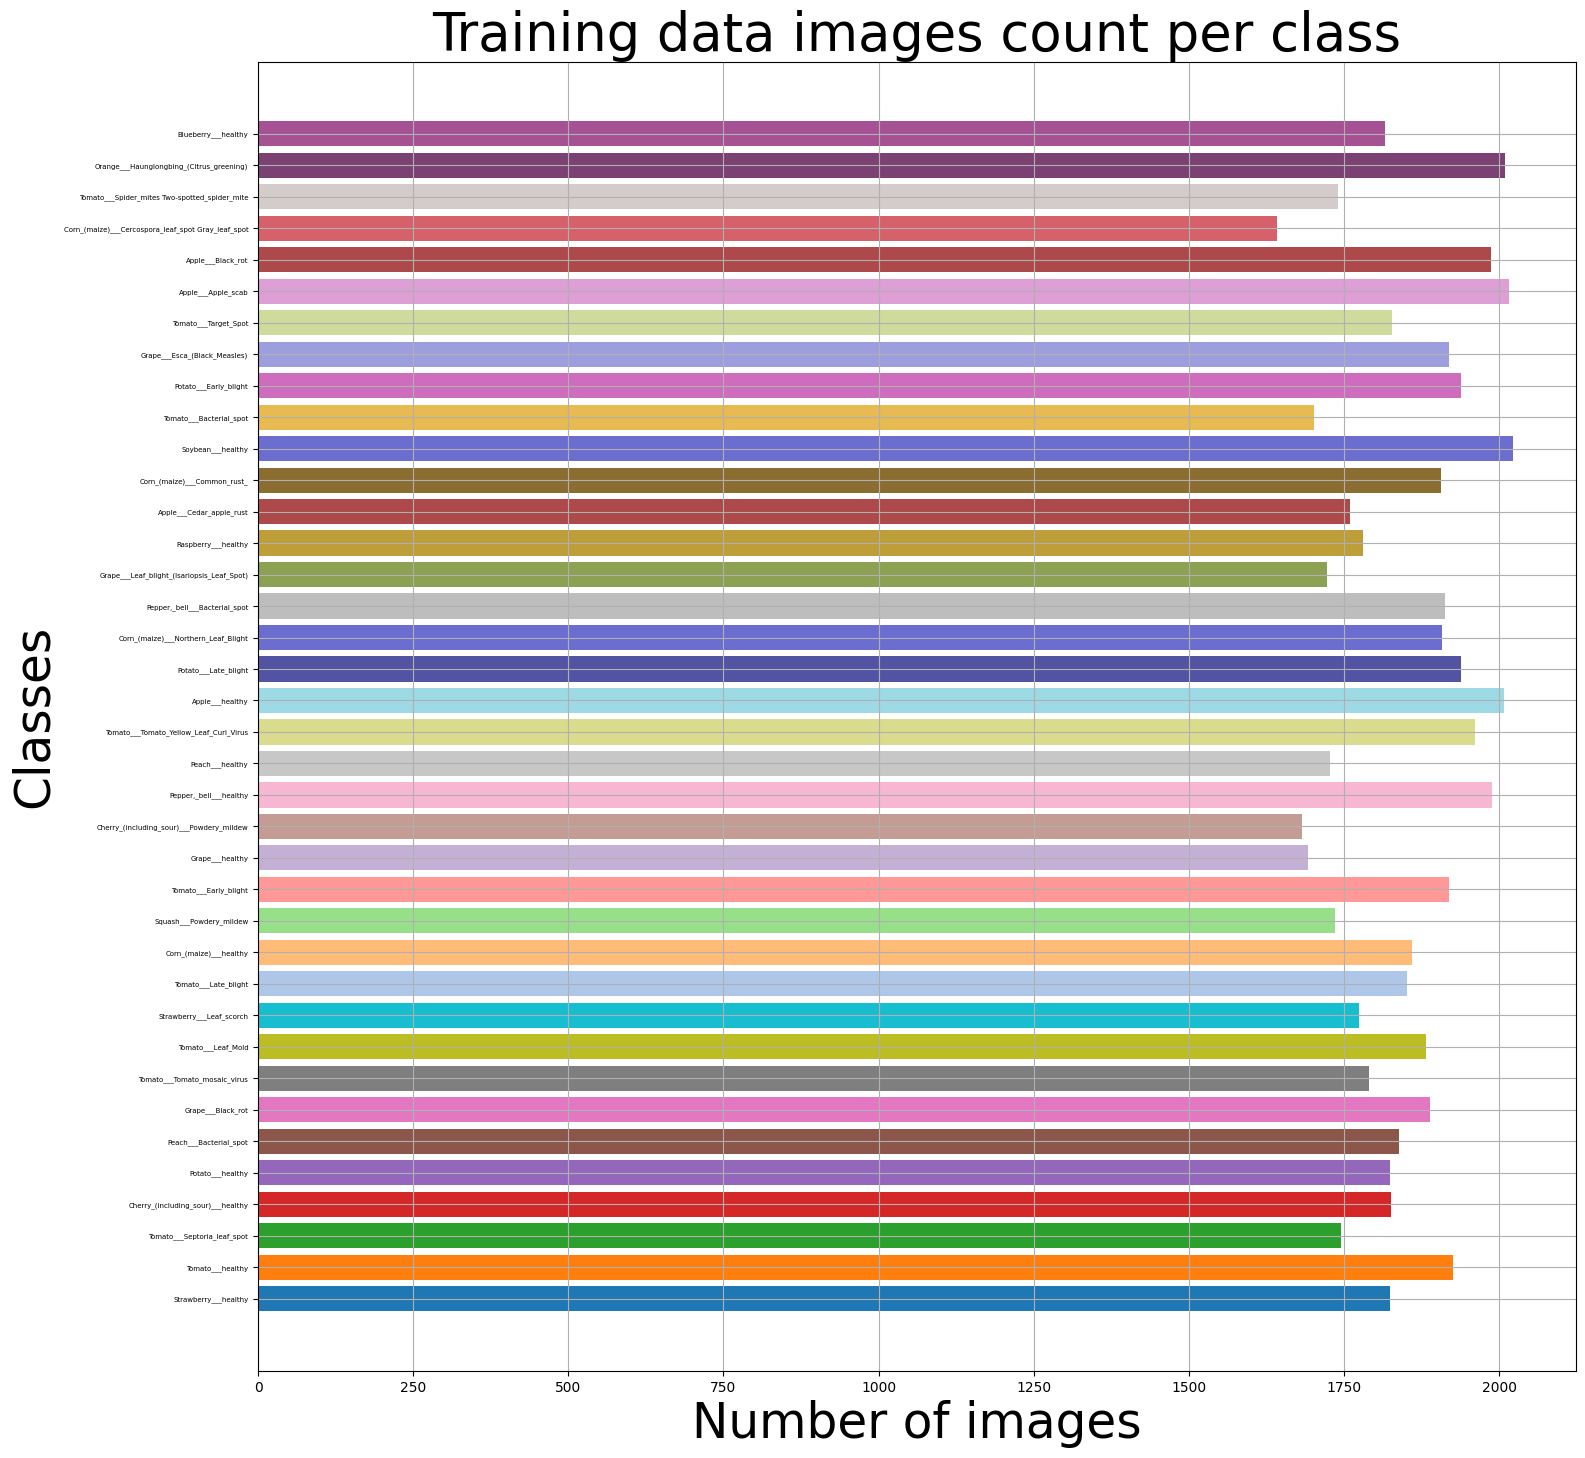
\includegraphics[width= 0.9\textwidth]{assets/class_distribution_big_leaves.png} 
    \caption{Class distribution} 
    \label{fig:immagine}
\end{figure}

As we can see the class distribution of the training dataset is quite balanced.

\chapter{Related Works}

In recent years, the application of Convolutional Neural Networks (CNNs) has revolutionized the field of image analysis, 
offering promising solutions to various problems, including the detection and diagnosis of plant diseases. 
Despite the success of CNNs, the challenges inherent in precise plant disease diagnosis persist and continue to drive 
research in this domain.

The recognition and classification of plant diseases from images is a complex task due to variations in plant species, 
environmental conditions, and the diverse manifestations of diseases. Researchers have made significant strides in 
addressing these challenges, and several noteworthy contributions in this area have advanced our understanding and 
capabilities.

\textbf{F. Marzougui, M. Elleuch and M. Kherallah} in their paper titled 
\textit{A Deep CNN Approach for Plant Disease Detection} \cite{Marzougui} presented an ensemble solution for plant 
disease diagnosis. They leveraged variants of classifiers designed with pretrained neural network architectures. 
Their approach achieved remarkable results, including a weighted F1-score of 97.2\% on the test dataset. 
% LINK: https://ieeexplore.ieee.org/document/9300072

\textbf{Nishant Shelar, Suraj Shinde, Shubham Sawant, Shreyash Dhumal and Kausar Fakir} in their publication 
\textit{Plant Disease Detection Using Cnn} \cite{NishantShelar} Their paper aims to develop a Disease Recognition 
Model using leaf image classification and convolutional neural networks (CNNs) for precise plant disease detection. 
CNNs are specialized for image processing and recognition, making them suitable for this task. 
Their model demonstrated a weighted F1-score of 95.6\% on the final test set.
% LINK https://www.itm-conferences.org/articles/itmconf/pdf/2022/04/itmconf_icacc2022_03049.pdf

\textbf{Shi, T., Liu, Y., Zheng,} explored 
\textit{Recent advances in plant disease severity assessment using convolutional neural networks} \cite{Shi}.
This study reviews 16 CNN-based approaches for severity assessment, discusses dataset acquisition, evaluation metrics, 
and addresses challenges, offering research ideas and solutions for practical applications. Additionally, 
they incorporated a basic attention mechanism to enhance their model's performance. Their ensemble of neural 
networks achieved a weighted F1-score of 98.7\% on the final test dataset.
% LINK: https://www.nature.com/articles/s41598-023-29230-7#citeas

\textbf{Hassan, S.M.; Maji, A.K.; Jasi `nski, M.; Leonowicz, Z.; Jasi `nska} introduced 
\textit{Identification of Plant-Leaf Diseases Using CNN and Transfer-Learning Approach} \cite{Hassan}, 
they optimized the models by using depth-separable convolution, reducing parameters and computation. 
With training on a diverse dataset, the models achieved high accuracy rates, surpassing traditional methods, 
and outperformed other deep-learning models, showing promise for efficient real-time disease detection in agriculture.
% LINK https://www.sciencedirect.com/science/article/abs/pii/S0168169917311742

Our project, \textit{Precision in Plant Disease Diagnosis: A CNN Approach to Enhance Agricultural Practices}, 
contributes to this body of work by evaluating the effectiveness of CNN models in plant disease detection. 
We aim to determine which approach, whether building a CNN from scratch or utilizing pre-trained weights, 
offers superior accuracy in plant disease diagnosis. Our efforts are geared towards advancing agricultural 
practices and promoting healthier crop yields.

\chapter{Methods and Experiments}

In this chapter, we discuss the implementation of a Convolutional Neural Network (CNN) model using TensorFlow 
and Keras for the purpose of image classification. The model has been trained over 20 epochs. This chapter provides 
a detailed breakdown of the code used for building and training the CNN.

\section{Neural Network From Scratch}

\subsection{Model Architecture}

The model architecture is structured as follows:

\subsubsection{Data Augmentation and Rescaling}
These are the layers used to apply changes to the images.

\paragraph{Data Augmentation}
A data augmentation layer is added to enhance the training dataset by applying random transformations to the input images.

\begin{lstlisting}[language=Python]
	data_augmentation = keras.Sequential([
	layers.RandomFlip("horizontal"), # Applies horizontal flipping to a random 50% of the images
	layers.RandomRotation(0.1), # Rotates the input images by a random value in the range[-10\%, +10\%] (fraction of full circle [-36, 36])
	layers.RandomZoom(0.1), # Zooms in or out of the image by a random factor in the range [-20%, +20%]
	layers.RandomContrast(0.1),
	],
	name = "AugmentationLayer"
	)
\end{lstlisting}

\begin{figure}[H]
    \centering
    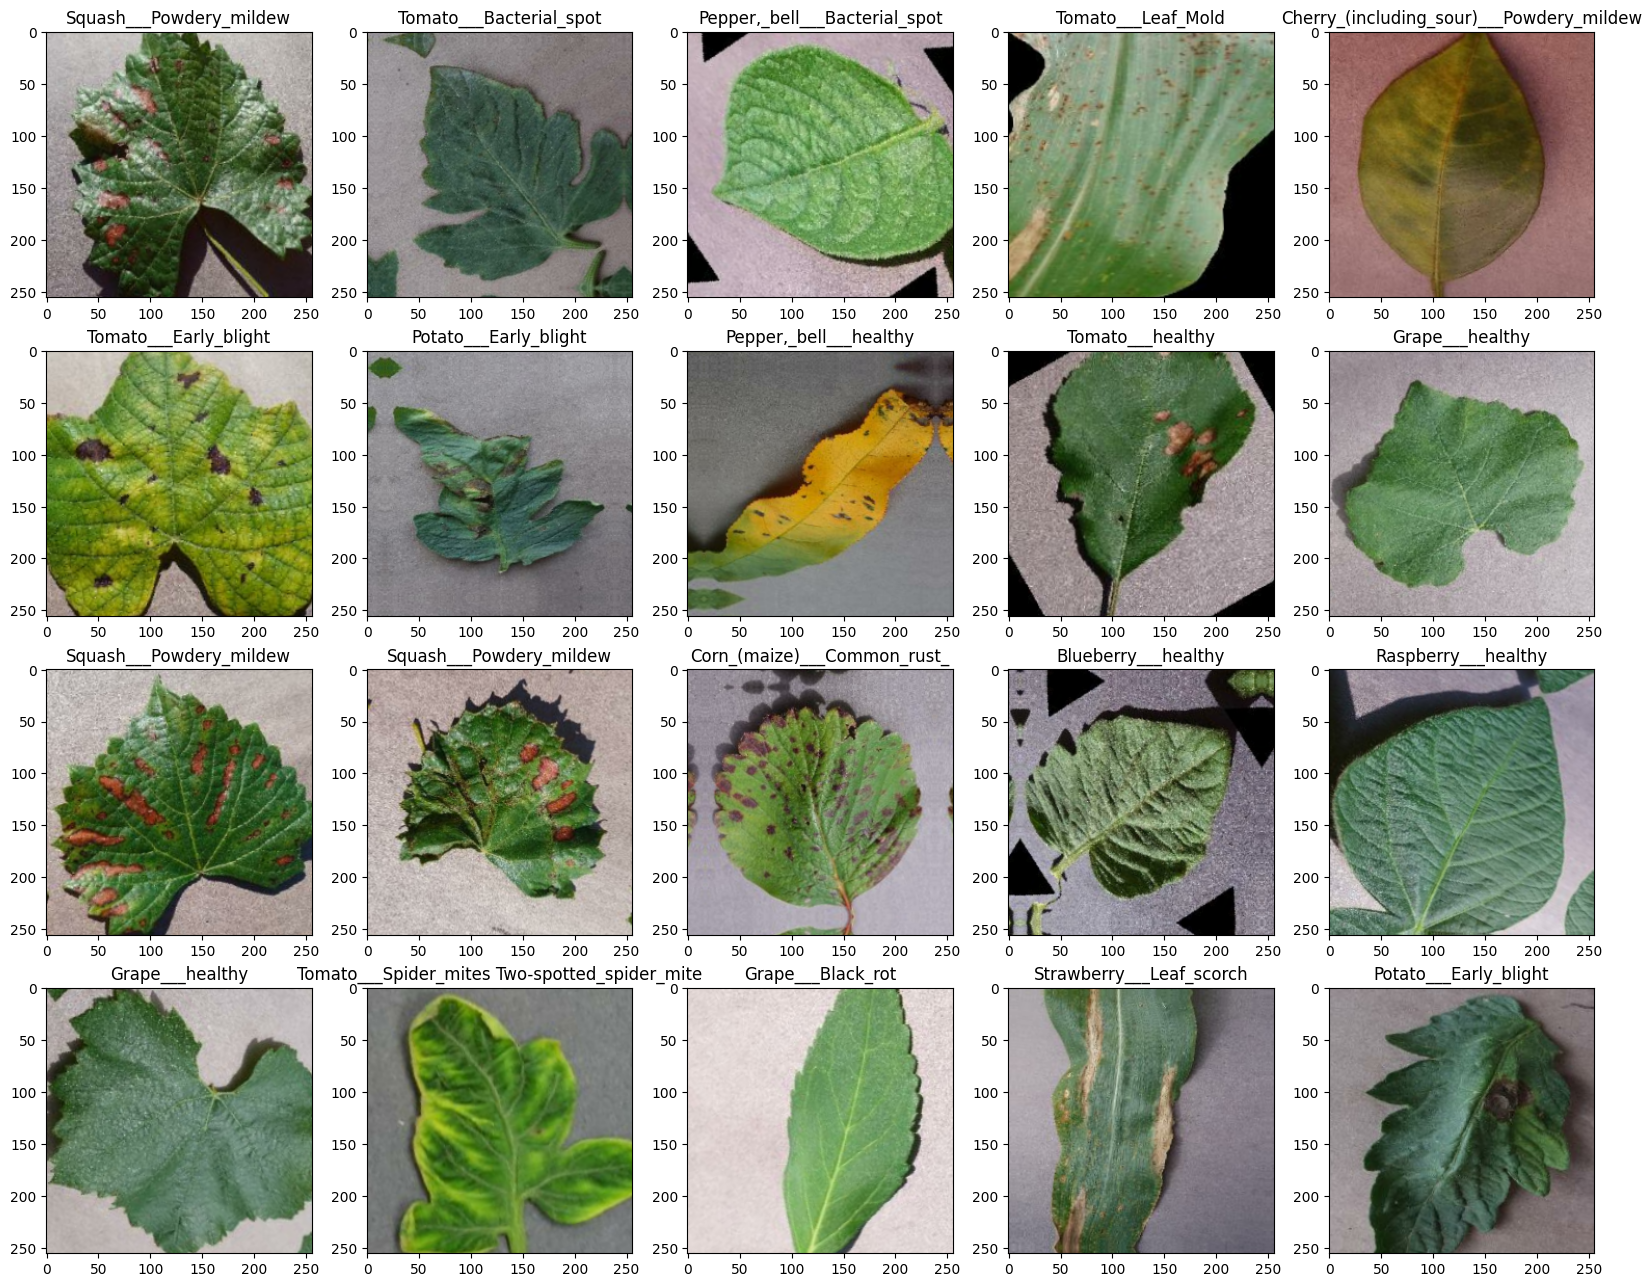
\includegraphics[width= 0.8\textwidth]{assets/augmentation.png} 
    \caption{Some of the augmented images} 
    \label{fig:immagine}
\end{figure}

\paragraph{Rescaling}

A rescaling layer is incorporated to normalize the pixel values to the range [0, 1].

\begin{lstlisting}[language=Python]
	model.add(layers.Rescaling(1./255))
\end{lstlisting}

\subsubsection{Convolutional Layers}
Multiple convolutional layers with varying numbers of filters, kernel sizes, and activation functions (ReLU) are 
introduced to extract features from the input images. Max-pooling and batch normalization layers are applied 
subsequently to downsample and normalize the feature maps.

\begin{lstlisting}[language=Python]
	model.add(layers.Conv2D(32, kernel_size = 3, activation = "relu6", padding = "same", input_shape = (256, 256,3)))
	model.add(layers.MaxPooling2D((2, 2)))
	model.add(layers.BatchNormalization())

	model.add(layers.Conv2D(64, kernel_size = 3, activation='relu', padding = "same"))
	model.add(layers.MaxPooling2D((2, 2)))
	model.add(layers.BatchNormalization())

	model.add(layers.Conv2D(128, kernel_size = 3, activation='relu', padding = "same"))
	model.add(layers.MaxPooling2D((2, 2)))
	model.add(layers.BatchNormalization())

	model.add(layers.Conv2D(256, kernel_size = 3, activation='relu', padding = "same"))
	model.add(layers.MaxPooling2D((2, 2)))
	model.add(layers.BatchNormalization())

	model.add(layers.Conv2D(512, kernel_size = 3, activation='relu', padding = "same"))
	model.add(layers.MaxPooling2D((2, 2)))
	model.add(layers.BatchNormalization())

	model.add(layers.Conv2D(512, kernel_size = 3, activation='relu', padding = "same"))
	model.add(layers.MaxPooling2D((2, 2)))
	model.add(layers.BatchNormalization())
\end{lstlisting}

Of course, this represents the final and most optimized model in our architecture. The model's composition began with 
just three building blocks, each consisting of a \textit{Conv2D} layer, a \textit{MaxPooling2D} layer, and a 
\textit{BatchNormalization} layer. In its initial form, the model included three chunks, each comprising 32, 64, and 128 
feature maps, respectively. As our experimentation progressed, we systematically added more chunks to the architecture 
to enhance the training accuracy.

\subsubsection{Top Layer}
It is responsible for adapting the network's output to the specific problem.

\paragraph{Flatten Layer}
A flatten layer is employed to convert the output from the convolutional layers into a 1D vector.

\begin{lstlisting}[language=Python]
	model.add(layers.Flatten())
\end{lstlisting}

\paragraph{Dropout Layer}
Dropout with a rate of 0.5 is used to regularize the model by randomly deactivating a portion of input units. It's 
used against overfitting.

\begin{lstlisting}[language=Python]
	model.add(layers.Dropout(0.5))
\end{lstlisting}

\paragraph{Dense Layers}
One fully connected (dense) layer with \textit{ReLU} activation function is added to facilitate the classification. The last 
layer is formed by the same number of neuron as the number of classes and it has the \textit{Softmax} activation function.

\begin{lstlisting}[language=Python]
	model.add(layers.Dense(256,activation="relu"))
	model.add(layers.Dense(38,activation="softmax"))
\end{lstlisting}

This is the resulting model:

\begin{table}[h]
	\centering
	\begin{tabular}{ccc}
	\hline
	\textbf{Layer}                & \textbf{Output Shape}      & \textbf{Param \#}    \\ 
	AugmentationLayer             & (None, 256, 256, 3)       & 0                    \\ 
	rescaling\_3                  & (None, 256, 256, 3)       & 0                    \\ 
	conv2d\_6                     & (None, 256, 256, 32)      & 896                  \\ 
	max\_pooling2d\_6             & (None, 128, 128, 32)      & 0                    \\ 
	batch\_normalization\_9       & (None, 128, 128, 32)      & 128                  \\ 
	conv2d\_7                     & (None, 128, 128, 64)      & 18496                \\ 
	max\_pooling2d\_7             & (None, 64, 64, 64)        & 0                    \\ 
	batch\_normalization\_10      & (None, 64, 64, 64)        & 256                  \\ 
	conv2d\_8                     & (None, 64, 64, 128)       & 73856                \\ 
	max\_pooling2d\_8             & (None, 32, 32, 128)       & 0                    \\ 
	batch\_normalization\_11      & (None, 32, 32, 128)       & 512                  \\ 
	conv2d\_9                     & (None, 32, 32, 256)       & 295168               \\ 
	max\_pooling2d\_9             & (None, 16, 16, 256)       & 0                    \\ 
	batch\_normalization\_12      & (None, 16, 16, 256)       & 1024                 \\ 
	conv2d\_10                    & (None, 16, 16, 512)       & 1180160              \\ 
	max\_pooling2d\_10            & (None, 8, 8, 512)         & 0                    \\ 
	batch\_normalization\_13      & (None, 8, 8, 512)         & 2048                 \\ 
	conv2d\_11                    & (None, 8, 8, 512)         & 2359808              \\ 
	max\_pooling2d\_11            & (None, 4, 4, 512)         & 0                    \\ 
	batch\_normalization\_14      & (None, 4, 4, 512)         & 2048                 \\ 
	flatten\_4                    & (None, 8192)              & 0                    \\ 
	dropout\_4                    & (None, 8192)              & 0                    \\ 
	dense\_8                      & (None, 256)               & 2097408              \\ 
	dense\_9                      & (None, 38)                & 9766                 \\ 
	\hline
	\end{tabular}
	\caption{From scratch model}
	\label{tab:model_details}
\end{table}

\subsection{Model Training}

The model is trained through the following steps:

\subsubsection{Compile Settings}
In this section we explain the settings chosen for the compilation of the model:
\begin{itemize}
	\item \textbf{loss}: we used \textit{categorical\_crossentropy} because it quantifies the dissimilarity 
		between predicted class probabilities and actual class labels. The formula for the categorical crossentropy
		is as follows: $-\sum_i{y_i \cdot log(p_i)}$ where $y_i$is the true probability distribution for class i and 
		$p_i$ is the predicted probability for class i as output by the model.
	\item \textbf{optimizer}: the algorithm used to update the model's weights during training is \textit{Adam}. We chose 
		this optimizer instead of \textit{rmsprop} because of his popularity and adaptive learning rates.
	\item \textbf{metrics}: we chose to use \textit{accuracy} as our metric due to the balanced dataset, its interpretability, 
		and the absence of a need to favor either FP or FN.
\end{itemize}

\begin{lstlisting}[language=Python]
	model.compile(
		loss="categorical_crossentropy",
		optimizer="adam",
		metrics=["accuracy"]
	)
\end{lstlisting}

\subsubsection{Callbacks}

The defined callbacks are \textbf{early stopping} and \textbf{model checkpoint}, to monitor the training process.

\begin{lstlisting}[language=Python]
	save_best_model = tf.keras.callbacks.ModelCheckpoint(modelPath, verbose=True, monitor='val_loss', save_best_only=True, save_weights_only=True)

	earlyStopping = tf.keras.callbacks.EarlyStopping(monitor='val_loss', patience=5)
\end{lstlisting}

\textit{ModelCheckpoint} callback is saving the best model weights based on validation loss, while the 
\textit{EarlyStopping} callback is stopping the training early if the validation loss doesn't improve over a 
specified number of epochs (in this case, 5 consecutive epochs). 

\subsubsection{Fitting}
The model is trained using the \texttt{model.fit()} method with the training and validation datasets. 
Training spans 20 epochs.

\begin{lstlisting}[language=Python]
	history = model.fit(
    train_dataset,
    epochs=20,
    validation_data=valid_dataset,
    validation_steps=len(valid_dataset),
    callbacks=[earlyStopping, save_best_model]
  )
\end{lstlisting}

\begin{figure}[H]
    \centering
    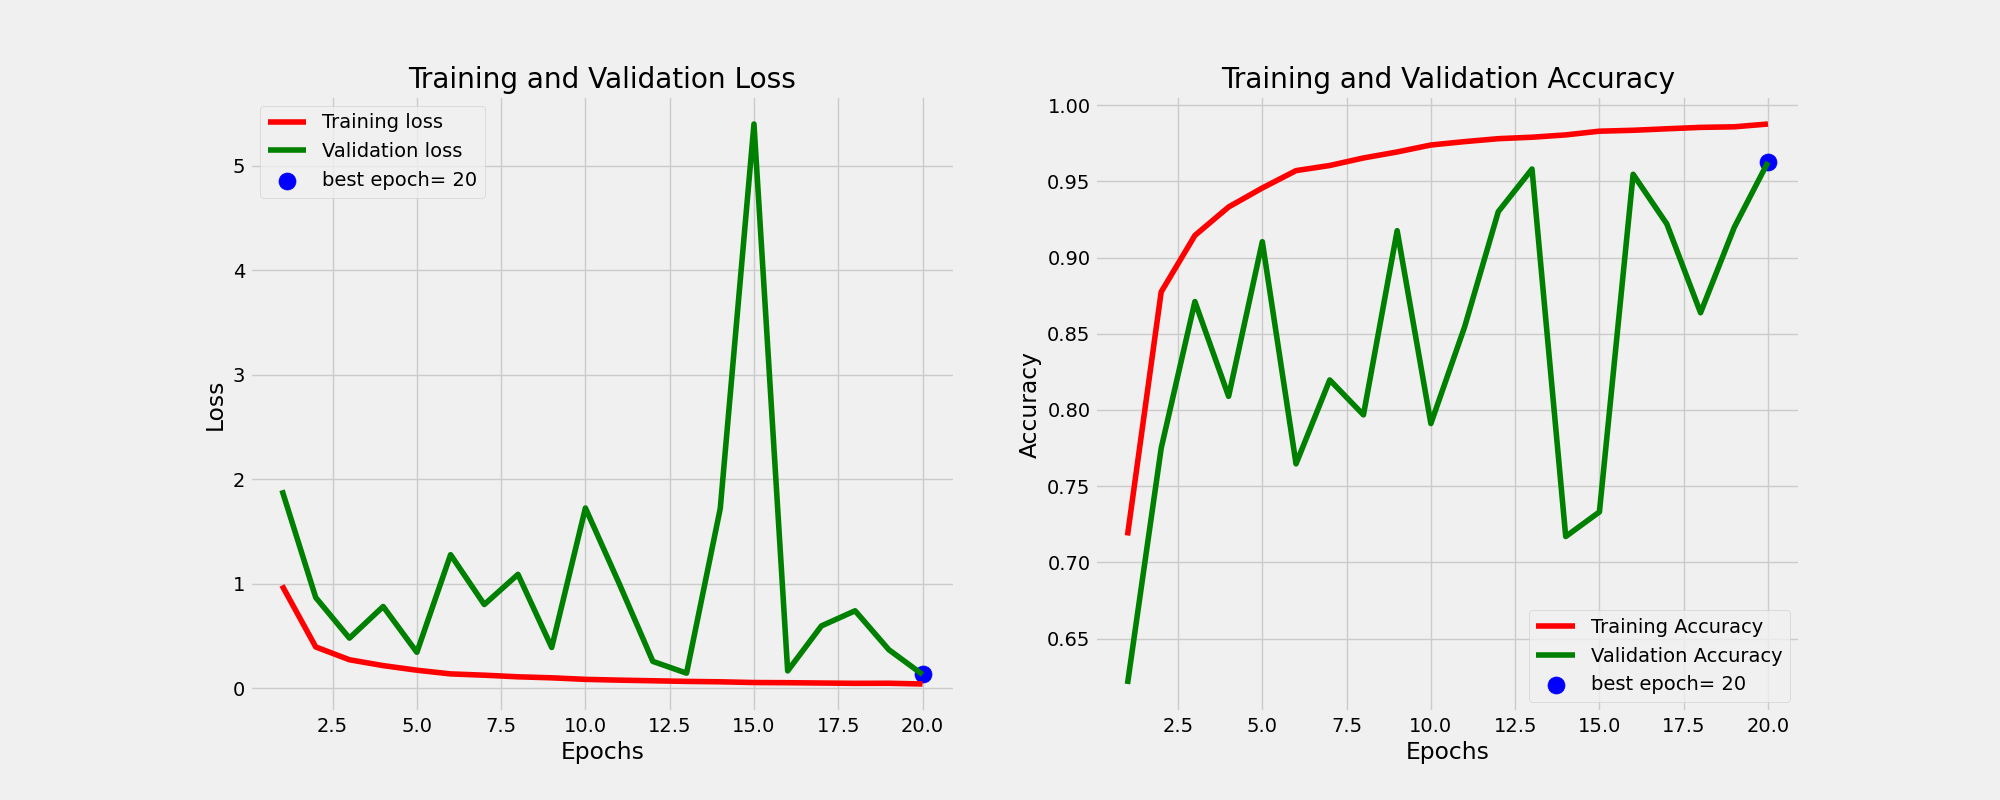
\includegraphics[width= 0.8\textwidth]{assets/scratch/32relu6_64_128_256_512_512_Drp_256d.png} 
    \caption{Training and Validation Accuracy/Loss of the model} 
    \label{fig:immagine}
\end{figure}

\section{Feature Extraction}

In our study, we explored various pretrained Convolutional Neural Network (CNN) models, such as EfficientNetV2L, 
EfficientNetB5, and EfficientNetB7. However, these complex models demanded substantial computational resources 
and time for training, ultimately falling short of our performance expectations.

Recognizing these challenges, we redirected our efforts toward a simpler CNN architecture, VGG16. This decision 
yielded significantly improved accuracy, highlighting that, in specific scenarios, simplicity can outperform 
complexity. By adopting VGG16, we streamlined our experimentation, optimized resource allocation, and ultimately 
achieved more satisfactory outcomes for our research objectives.

\begin{figure}[H]
    \centering
    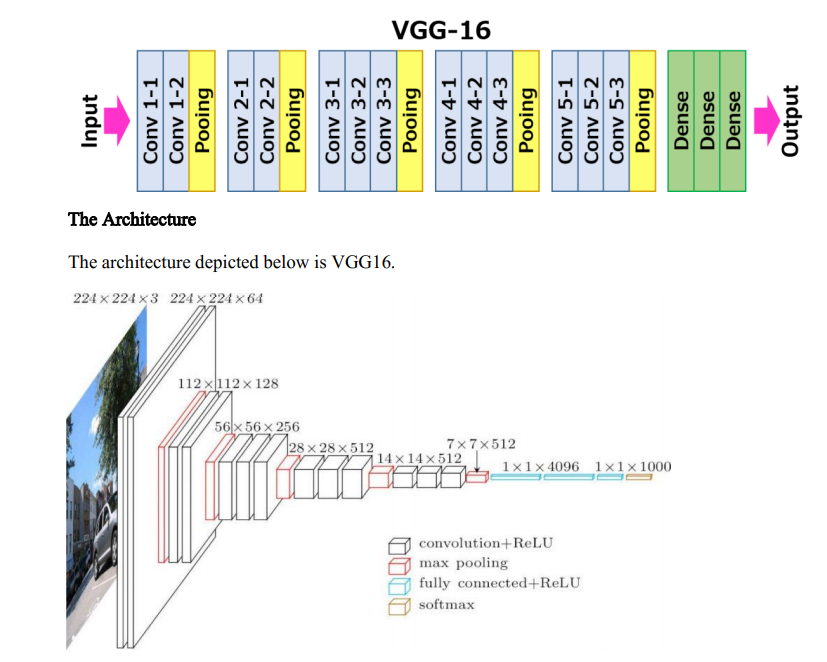
\includegraphics[width= 0.8\textwidth]{assets/VGG16.png} 
    \caption{VGG16 architecture} 
    \label{fig:immagine}
\end{figure}

\subsection{Defining the CNN Model}

Below is the code to define the CNN model based on VGG16:

\begin{lstlisting}[language=Python]
	# Define a CNN model based on pre-trained VGG16
	cnn_base = tf.keras.applications.VGG16(
	include_top=False,           # Do not include the fully connected layer on top of the model
	weights="imagenet",          # Use pre-trained weights from ImageNet
	input_shape=(IMAGE_HEIGHT, IMAGE_WIDTH, 3),  # Specify input shape (height, width, channels)
	pooling='max',               # Use max-pooling as the pooling operation
	)
\end{lstlisting}

In this implementation, we have used several key parameters to configure the VGG16 model according to our needs.

\subsubsection{Parameter \textit{include\_top}}
The \textit{include\_top} parameter is set to `False`, which means we will not include the fully connected layer at the 
top of the VGG16 model. This is useful when we intend to add our own layers on top to adapt the model for our specific tasks.

\subsubsection{Parameter \textit{weights}}
The \textit{weights} parameter is set to "imagenet," indicating that we are using pre-trained weights of the VGG16
model trained on ImageNet. This choice allows us to benefit from the knowledge learned by the network on a large dataset.

\subsubsection{Parameter \textit{input\_shape}}
We defined the input\_shape parameter to specify the expected dimensions of the input that the model accepts. 
Both IMAGE\_HEIGHT and IMAGE\_WIDTH are set to 256. The value 3 signifies the number of channels for RGB images.

\subsubsection{Parameter \textit{pooling}}
The \textit{pooling} parameter is set to "max", indicating the use of max-pooling as the pooling operation after the 
convolutional layers. Max-pooling is used to reduce the size of feature maps.


\subsection{Image Preprocessing and Convolutional Base}

In this section, we'll discuss image preprocessing and the configuration of the convolutional base.

\subsubsection{Image Preprocessing}

We create a sequential model for resizing and rescaling images:

\begin{lstlisting}[language=Python]
	resize_and_rescale = tf.keras.Sequential([
	layers.Resizing(IMAGE_HEIGHT, IMAGE_WIDTH), # Resize input images
	layers.Rescaling(1./255)  # Rescale pixel values to [0, 1]
	])
\end{lstlisting}

This sequential model consists of two layers. The first layer, \textbf{layers.Resizing}, resizes input images to the 
specified dimensions of \texttt{IMAGE\_HEIGHT} and \texttt{IMAGE\_WIDTH}. The second layer, \textbf{layers.Rescaling}, 
scales the pixel values of the images to the range [0, 1].

\subsubsection{Layers Freezing}

We set the convolutional base (\texttt{cnn\_base}) to be non-trainable:

	\begin{lstlisting}[language=Python]
		cnn_base.trainable = False
	\end{lstlisting}

This line ensures that the convolutional layers within the \texttt{cnn\_base} model will not receive updates 
during training. Only the additional layers added on top of it will be trained.

\subsection{Building and Compiling the Pretrained Model}

In this section, we'll discuss the construction and compilation of the pretrained model.

\subsubsection{Model Architecture}

We construct a sequential model by stacking various layers:

\begin{lstlisting}[language=Python]
	pretrained_model = tf.keras.Sequential([
	resize_and_rescale,  # Image preprocessing and rescaling
	data_augmentation,   # Data augmentation for training
	cnn_base,            # Pretrained convolutional base
	layers.Flatten(),    # Flatten feature maps
	layers.Dense(256, activation="relu"),  # Fully connected layer with ReLU activation
	layers.BatchNormalization(),           # Batch normalization layer
	layers.Dropout(0.4),                   # Dropout layer with 40% dropout rate
	layers.Dense(38, activation="softmax") # Output layer with softmax activation
	])
\end{lstlisting}

\paragraph{resize\_and\_rescale} This is the image preprocessing and rescaling step that we discussed earlier.

\paragraph{data\_augmentation} Data augmentation is used for training, and it helps generate variations of the 
	training data to improve model generalization.

\paragraph{cnn\_base} The pretrained convolutional base, which was frozen earlier, serves as the feature extractor.

\paragraph{layers.Flatten()} This layer is used to flatten the feature maps from the convolutional base.

\paragraph{layers.Dense(256, activation="relu")} A fully connected layer with 256 units and ReLU activation.

\paragraph{layers.BatchNormalization()} A batch normalization layer to normalize activations.

\paragraph{layers.Dropout(0.4)} A dropout layer with a dropout rate of 40\% to prevent overfitting.

\paragraph{layers.Dense(38, activation="softmax")} The output layer with softmax activation for multi-class classification. 
	The number of units (38) should match the number of classes.

\begin{table}[h]
	\centering
	\begin{tabular}{ccc}
	\hline
	\textbf{Layer (type)}          & \textbf{Output Shape} & \textbf{Param \#}     \\ 
	sequential\_4 (Sequential)     & (None, 256, 256, 3)  & 0                     \\ 
	AugmentationLayer (Sequential) & (None, 256, 256, 3)  & 0                     \\ 
	vgg16 (Functional)             & (None, 512)          & 14714688              \\ 
	flatten\_3 (Flatten)           & (None, 512)          & 0                     \\ 
	dense\_6 (Dense)               & (None, 256)          & 131328                \\ 
	batch\_normalization\_8        & (None, 256)          & 1024                  \\ 
	dropout\_3 (Dropout)           & (None, 256)          & 0                     \\ 
	dense\_7 (Dense)               & (None, 38)           & 9766                  \\ 
	\hline
	\end{tabular}
	\caption{Feature Extraction model}
	\label{tab:model_details}
\end{table}
	

We then proceeded following the same steps as the Neural Network from scratch.

\begin{figure}[H]
    \centering
    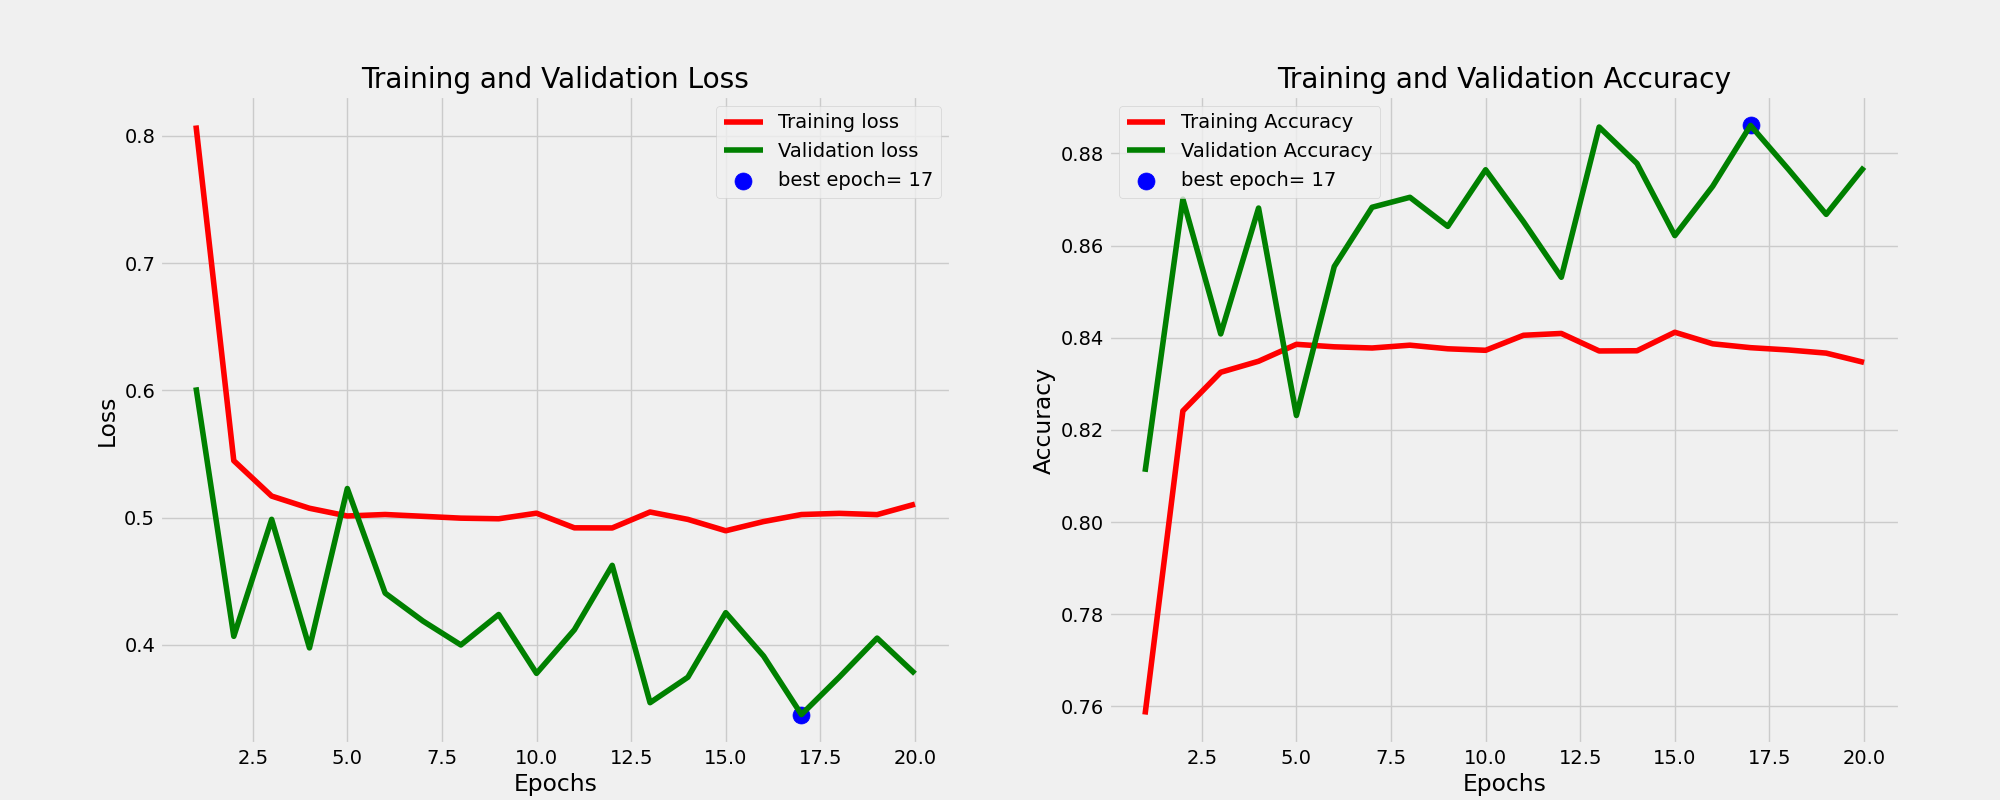
\includegraphics[width= 0.8\textwidth]{assets/FExtraction/FE_base_256d.png} 
    \caption{Training and Validation Accuracy/Loss of the model} 
    \label{fig:immagine}
\end{figure}

\section{Fine-Tuning}

In this section, we will explore the fine-tuning technique for building a Convolutional Neural Network. 
It's worth noting that some of the steps involved in constructing a fine-tuned CNN overlap with the steps used for 
feature extraction in the previously trained model. We will continue with the following steps:

\subsection{Layers Unfreezing}

Next, we unfreeze the last block of VGG16's convolutional layers:

\begin{lstlisting}[language=Python]
	# Allow training of the entire `cnn_base`
	cnn_base.trainable = True
	
	# Initialize a flag `set_trainable` to False
	set_trainable = False
	
	# Loop through the layers of the `cnn_base`
	for layer in cnn_base.layers:
		# Check if the layer name is 'block5_conv1'
		if layer.name == 'block5_conv1':
			set_trainable = True
		
		# If `set_trainable` is True, make the layer trainable; otherwise, freeze it
		if set_trainable:
			layer.trainable = True
		else:
			layer.trainable = False

\end{lstlisting}

\subsection{Model Compilation}

As for the other models we compile it with an important difference:

\begin{lstlisting}[language=Python]
	pretrained_model.compile(
	loss='categorical_crossentropy',  # Categorical cross-entropy loss
	optimizer=tf.keras.optimizers.Adam(learning_rate=0.00001),  # Adam optimizer with a custom learning rate
	metrics=["accuracy"]  # Accuracy metric for evaluation
	)
\end{lstlisting}

The learning rate is equal to 0.00001, this is used to retain valuable features learned during initial training, 
prevent overfitting, ensure stability, and enable fine-grained adjustments.

\subsection{Fine-Tuning Configuration}

We proceed with fine-tuning and configure callbacks for the process:

\begin{lstlisting}[language=Python]
	# Define the model name for fine-tuning
	modelName = "FT_base_256d"
	
	# Construct the model path for saving
	modelPath = os.path.join(fineTunedPath, modelName + ".keras")
	
	# Configure ModelCheckpoint callback
	save_best_model = tf.keras.callbacks.ModelCheckpoint(
	modelPath,
	monitor='val_loss', verbose=1,
	save_best_only=True, save_weights_only=True
	)
	
	# Configure EarlyStopping callback
	earlyStopping = tf.keras.callbacks.EarlyStopping(
	monitor='val_loss', patience=5
	)
\end{lstlisting}

\begin{figure}[H]
    \centering
    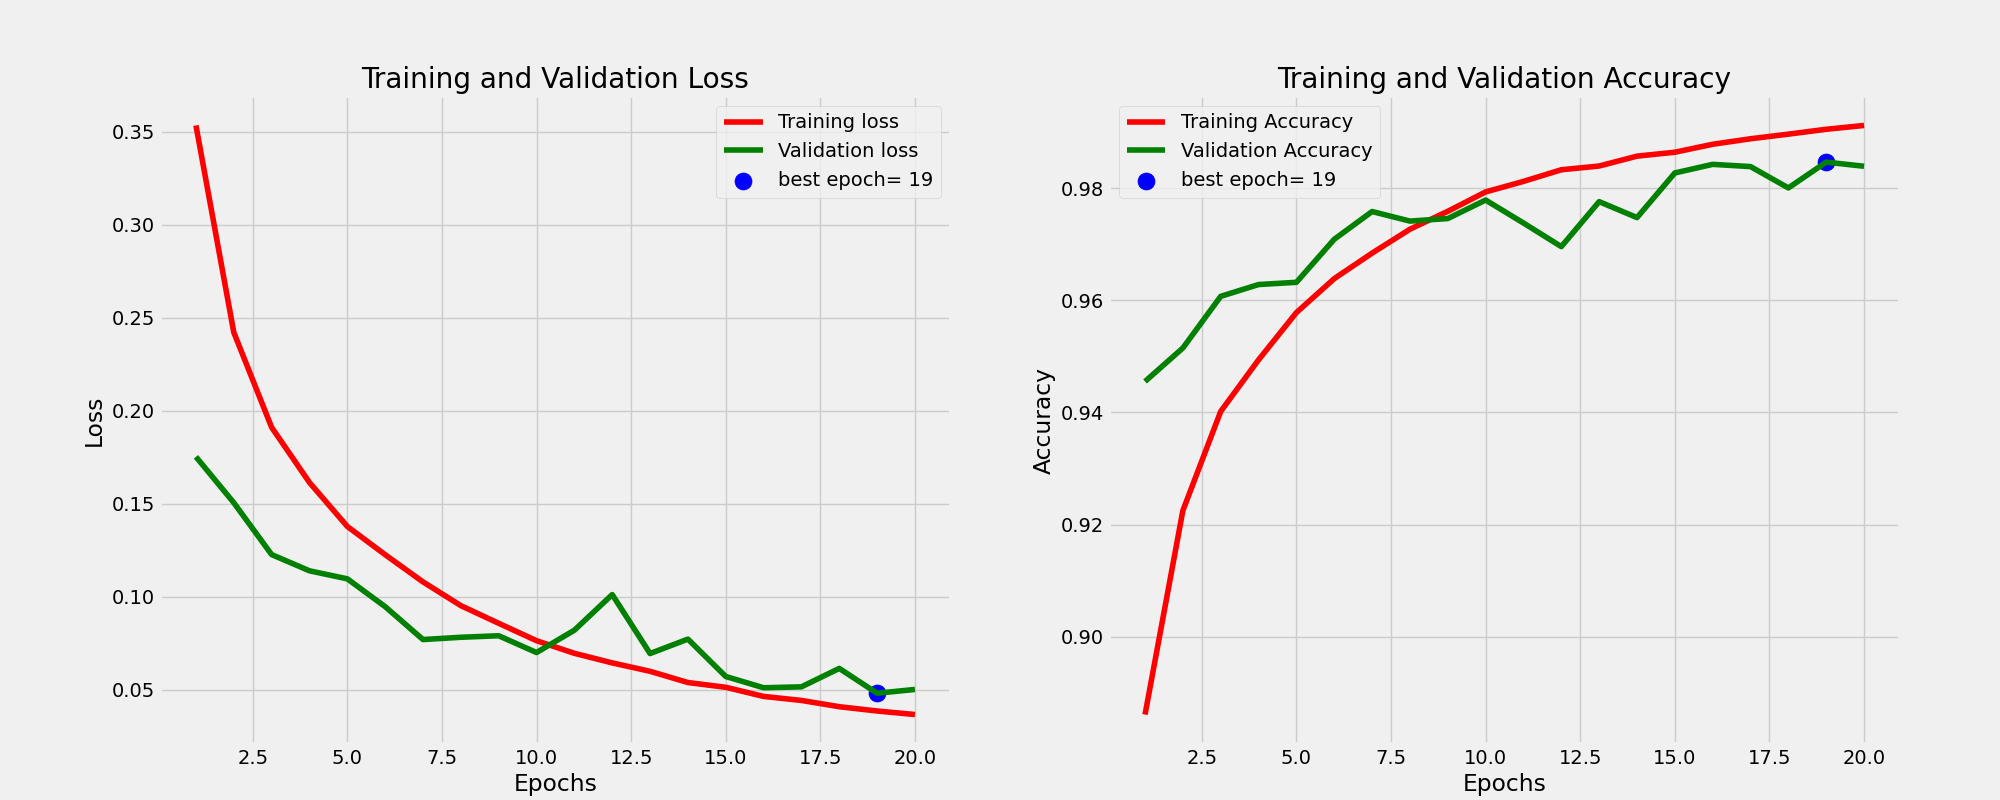
\includegraphics[width= 0.8\textwidth]{assets/fine-tuning/FT_base_256d.png} 
    \caption{Training and Validation Accuracy/Loss of the model} 
    \label{fig:immagine}
\end{figure}
\chapter{Results}
In conclusion these are the results of our resulting models applied on the test set.
Note that the tests are made only on the model from scratch and the fine-tuned one, because the feature extraction
one underperforms in every way in comparison of the fine-tuned model. 

\section{From Scratch Model}

\begin{table}[H]
	\centering
	\begin{tabular}{|l|c|}
		\hline
		\textbf{From scratch} & \\
		\hline
		Test Loss & 0.08954 \\
		Test Accuracy & 97.59\% \\
		\hline
	\end{tabular}
    \caption{Numerical accuracy and loss}
\end{table}

\begin{table}[H]
	\centering
	\begin{tabular}{lcccc}
		\hline
		\textbf{Class} & \textbf{Precision} & \textbf{Recall} & \textbf{F1-Score} & \textbf{Support} \\
		\hline
		Strawberry\_healthy & 1.00 & 0.89 & 0.94 & 63 \\
		Tomato\_healthy & 0.93 & 1.00 & 0.96 & 62 \\
		Tomato\_Septoria\_leaf\_spot & 1.00 & 1.00 & 1.00 & 28 \\
		Cherry\_healthy & 0.98 & 0.98 & 0.98 & 165 \\
		Potato\_healthy & 0.96 & 1.00 & 0.98 & 150 \\
		Peach\_Bacterial\_spot & 1.00 & 1.00 & 1.00 & 105 \\
		Grape\_Black\_rot & 0.86 & 1.00 & 0.92 & 86 \\
		Tomato\_Tomato\_mosaic\_virus & 0.85 & 1.00 & 0.92 & 52 \\
		Tomato\_Leaf\_Mold & 1.00 & 1.00 & 1.00 & 119 \\
		Strawberry\_Leaf\_scorch & 0.99 & 0.92 & 0.95 & 99 \\
		Tomato\_Late\_blight & 1.00 & 1.00 & 1.00 & 116 \\
		Corn\_healthy & 0.94 & 1.00 & 0.97 & 118 \\
		Squash\_Powdery\_mildew & 1.00 & 0.99 & 1.00 & 139 \\
		Tomato\_Early\_blight & 0.99 & 1.00 & 1.00 & 108 \\
		Grape\_healthy & 0.98 & 0.98 & 0.98 & 43 \\
		Cherry\_Powdery\_mildew & 1.00 & 1.00 & 1.00 & 551 \\
		Pepper\_bell\_healthy & 0.99 & 0.98 & 0.99 & 230 \\
		Peach\_healthy & 0.97 & 0.97 & 0.97 & 36 \\
		Tomato\_Tomato\_Yellow\_Leaf\_Curl\_Virus & 0.94 & 0.99 & 0.97 & 100 \\
		Apple\_healthy & 0.99 & 0.99 & 0.99 & 148 \\
		Potato\_Late\_blight & 0.98 & 1.00 & 0.99 & 100 \\
		Corn\_Northern\_Leaf\_Blight & 1.00 & 0.95 & 0.97 & 100 \\
		Pepper\_bell\_Bacterial\_spot & 0.88 & 0.47 & 0.61 & 15 \\
		Grape\_Leaf\_blight & 0.97 & 0.97 & 0.97 & 37 \\
		Raspberry\_healthy & 0.98 & 0.99 & 0.99 & 509 \\
		Apple\_Cedar\_apple\_rust & 1.00 & 0.99 & 0.99 & 184 \\
		Corn\_Common\_rust & 0.99 & 1.00 & 1.00 & 111 \\
		Soybean\_healthy & 0.96 & 0.98 & 0.97 & 46 \\
		Tomato\_Bacterial\_spot & 0.98 & 0.97 & 0.97 & 213 \\
		Potato\_Early\_blight & 0.96 & 0.94 & 0.95 & 100 \\
		Grape\_Esca & 0.99 & 0.93 & 0.96 & 191 \\
		Tomato\_Target\_Spot & 0.97 & 0.99 & 0.98 & 95 \\
		Apple\_Apple\_scab & 0.99 & 0.88 & 0.93 & 177 \\
		Blueberry\_healthy & 0.93 & 1.00 & 0.96 & 159 \\
		\hline
		\textbf{Accuracy} & & & 0.98 & 5438 \\
		\textbf{Macro Avg} & 0.97 & 0.96 & 0.96 & 5438 \\
		\textbf{Weighted Avg} & 0.98 & 0.98 & 0.98 & 5438 \\
		\hline
	\end{tabular}
	\caption{Classification Report}
\end{table}

\begin{figure}[H]
    \centering
    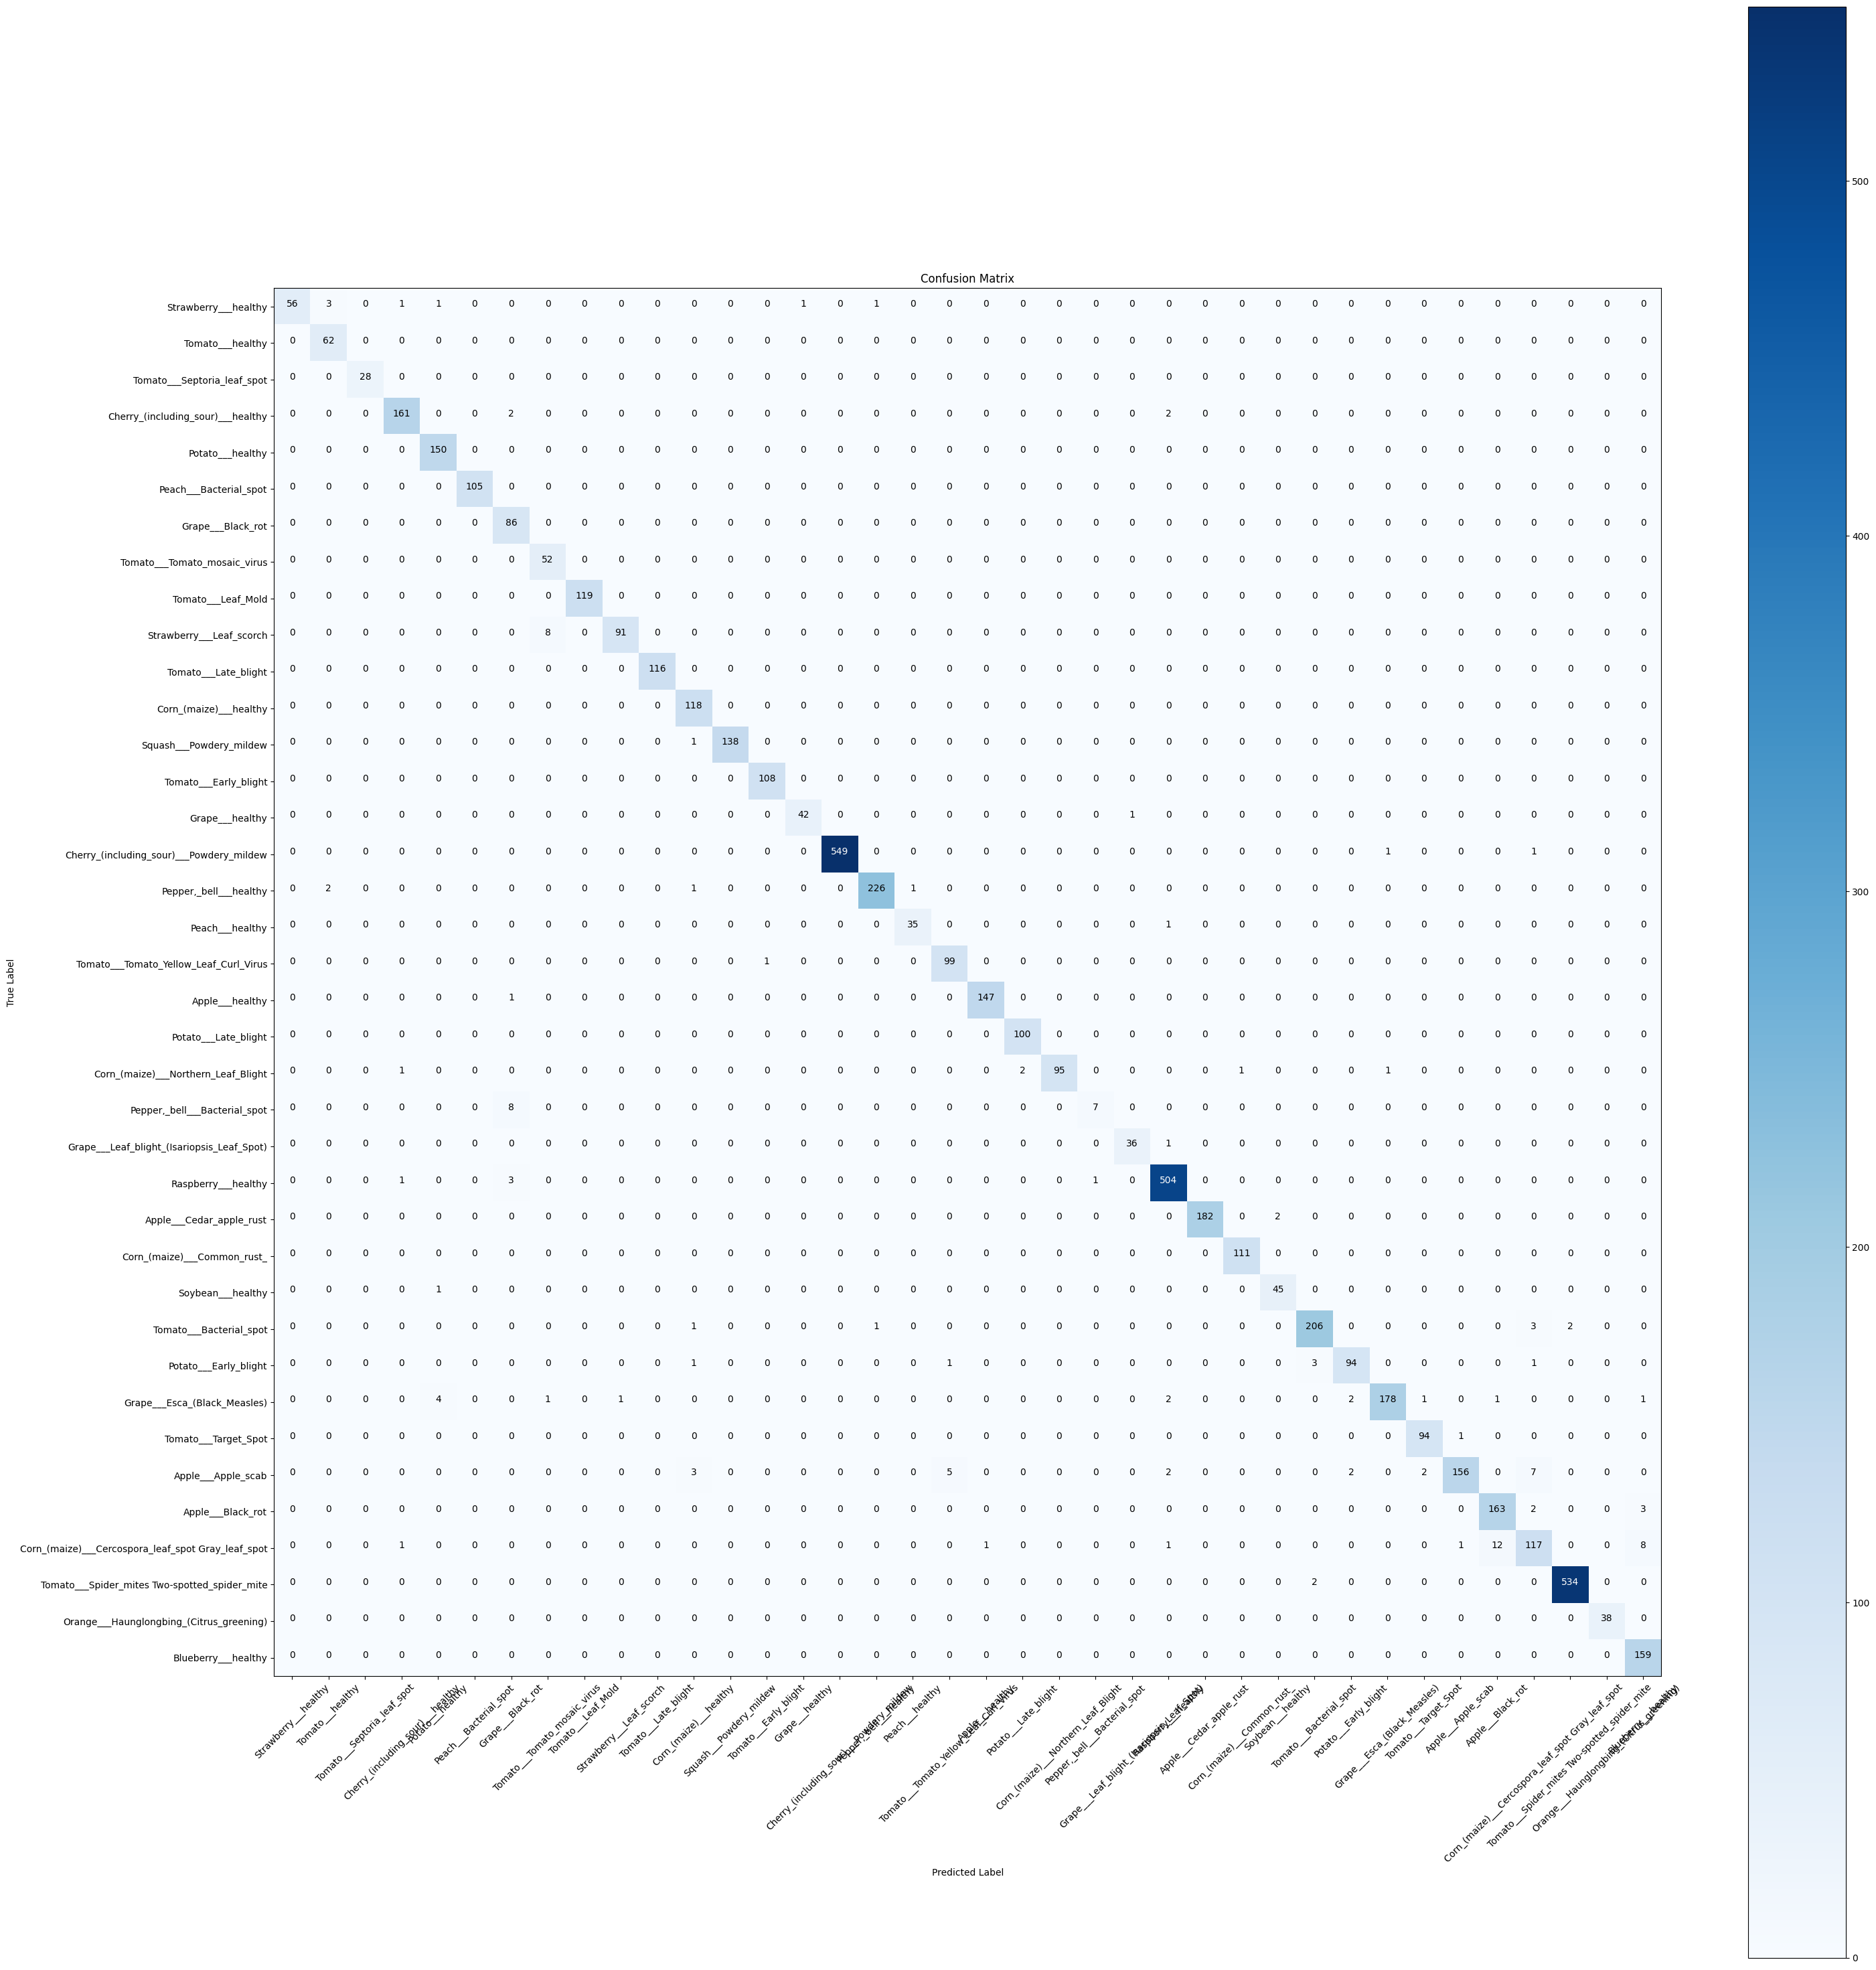
\includegraphics[width= 0.9\textwidth]{assets/FSConfMatrix.png} 
    \caption{Confusion Matrix} 
    \label{fig:immagine}
\end{figure}

Analysis of the confusion matrix and the F1-scores for individual classes reveals that the class posing the most significant
challenge is \textit{Pepper\_bell\_Bacterial\_spot}, with an F1-score of 61\% (notably, the lowest recall at 47\%). 
This issue may primarily stem from the limited availability of images for this particular class. This hypothesis 
gains support when considering that all other classes, benefiting from more extensive support, consistently 
perform at a significantly higher level, consistently exceeding a 90\% F1-score.

\section{Fine Tuned Model}

\begin{table}[H]
    \centering
    \begin{tabular}{|l|c|}
        \hline
        \textbf{Fine Tuned} & \\
        \hline
            Test Loss & 0.03156 \\
            \hline
            Test Accuracy & 99.01\% \\
            \hline
        \end{tabular}
     \caption{Numerical accuracy and loss}
\end{table}

\begin{table}[H]
	\centering
	\begin{tabular}{lcccc}
		\hline
		\textbf{Class} & \textbf{Precision} & \textbf{Recall} & \textbf{F1-Score} & \textbf{Support} \\
		\hline
		Strawberry\_healthy & 1.00 & 0.98 & 0.99 & 63 \\
		Tomato\_healthy & 1.00 & 1.00 & 1.00 & 62 \\
		Tomato\_Septoria\_leaf\_spot & 1.00 & 1.00 & 1.00 & 28 \\
		Cherry\_healthy & 1.00 & 0.99 & 1.00 & 165 \\
		Potato\_healthy & 1.00 & 1.00 & 1.00 & 150 \\
		Peach\_Bacterial\_spot & 1.00 & 1.00 & 1.00 & 105 \\
		Grape\_Black\_rot & 1.00 & 1.00 & 1.00 & 86 \\
		Tomato\_Tomato\_mosaic\_virus & 0.98 & 0.94 & 0.96 & 52 \\
		Tomato\_Leaf\_Mold & 1.00 & 1.00 & 1.00 & 119 \\
		Strawberry\_Leaf\_scorch & 0.96 & 0.99 & 0.98 & 99 \\
		Tomato\_Late\_blight & 1.00 & 1.00 & 1.00 & 116 \\
		Corn\_healthy & 1.00 & 1.00 & 1.00 & 118 \\
		Squash\_Powdery\_mildew & 1.00 & 1.00 & 1.00 & 139 \\
		Tomato\_Early\_blight & 1.00 & 1.00 & 1.00 & 108 \\
		Grape\_healthy & 1.00 & 1.00 & 1.00 & 43 \\
		Cherry\_Powdery\_mildew & 1.00 & 1.00 & 1.00 & 551 \\
		Pepper\_bell\_healthy & 0.99 & 0.98 & 0.99 & 230 \\
		Peach\_healthy & 0.88 & 1.00 & 0.94 & 36 \\
		Tomato\_Tomato\_Yellow\_Leaf\_Curl\_Virus & 1.00 & 0.99 & 0.99 & 100 \\
		Apple\_healthy & 0.99 & 1.00 & 1.00 & 148 \\
		Potato\_Late\_blight & 0.99 & 1.00 & 1.00 & 100 \\
		Corn\_Northern\_Leaf\_Blight & 1.00 & 0.94 & 0.97 & 100 \\
		Pepper\_bell\_Bacterial\_spot & 0.71 & 1.00 & 0.83 & 15 \\
		Grape\_Leaf\_blight & 1.00 & 1.00 & 1.00 & 37 \\
		Raspberry\_healthy & 1.00 & 1.00 & 1.00 & 509 \\
		Apple\_Cedar\_apple\_rust & 0.99 & 1.00 & 1.00 & 184 \\
		Corn\_Common\_rust & 1.00 & 1.00 & 1.00 & 111 \\
		Soybean\_healthy & 1.00 & 1.00 & 1.00 & 46 \\
		Tomato\_Bacterial\_spot & 1.00 & 1.00 & 1.00 & 213 \\
		Potato\_Early\_blight & 1.00 & 0.94 & 0.97 & 100 \\
		Grape\_Esca & 0.98 & 0.98 & 0.98 & 191 \\
		Tomato\_Target\_Spot & 1.00 & 0.88 & 0.94 & 95 \\
		Apple\_Apple\_scab & 0.99 & 0.98 & 0.99 & 177 \\
		Blueberry\_healthy & 0.99 & 1.00 & 0.99 & 159 \\
		\hline
		\textbf{Accuracy} & & & 0.99 & 5438 \\
		\textbf{Macro Avg} & 0.98 & 0.99 & 0.98 & 5438 \\
		\textbf{Weighted Avg} & 0.99 & 0.99 & 0.99 & 5438 \\
		\hline
	\end{tabular}
	\caption{Classification Report}
\end{table}

\begin{figure}[H]
    \centering
    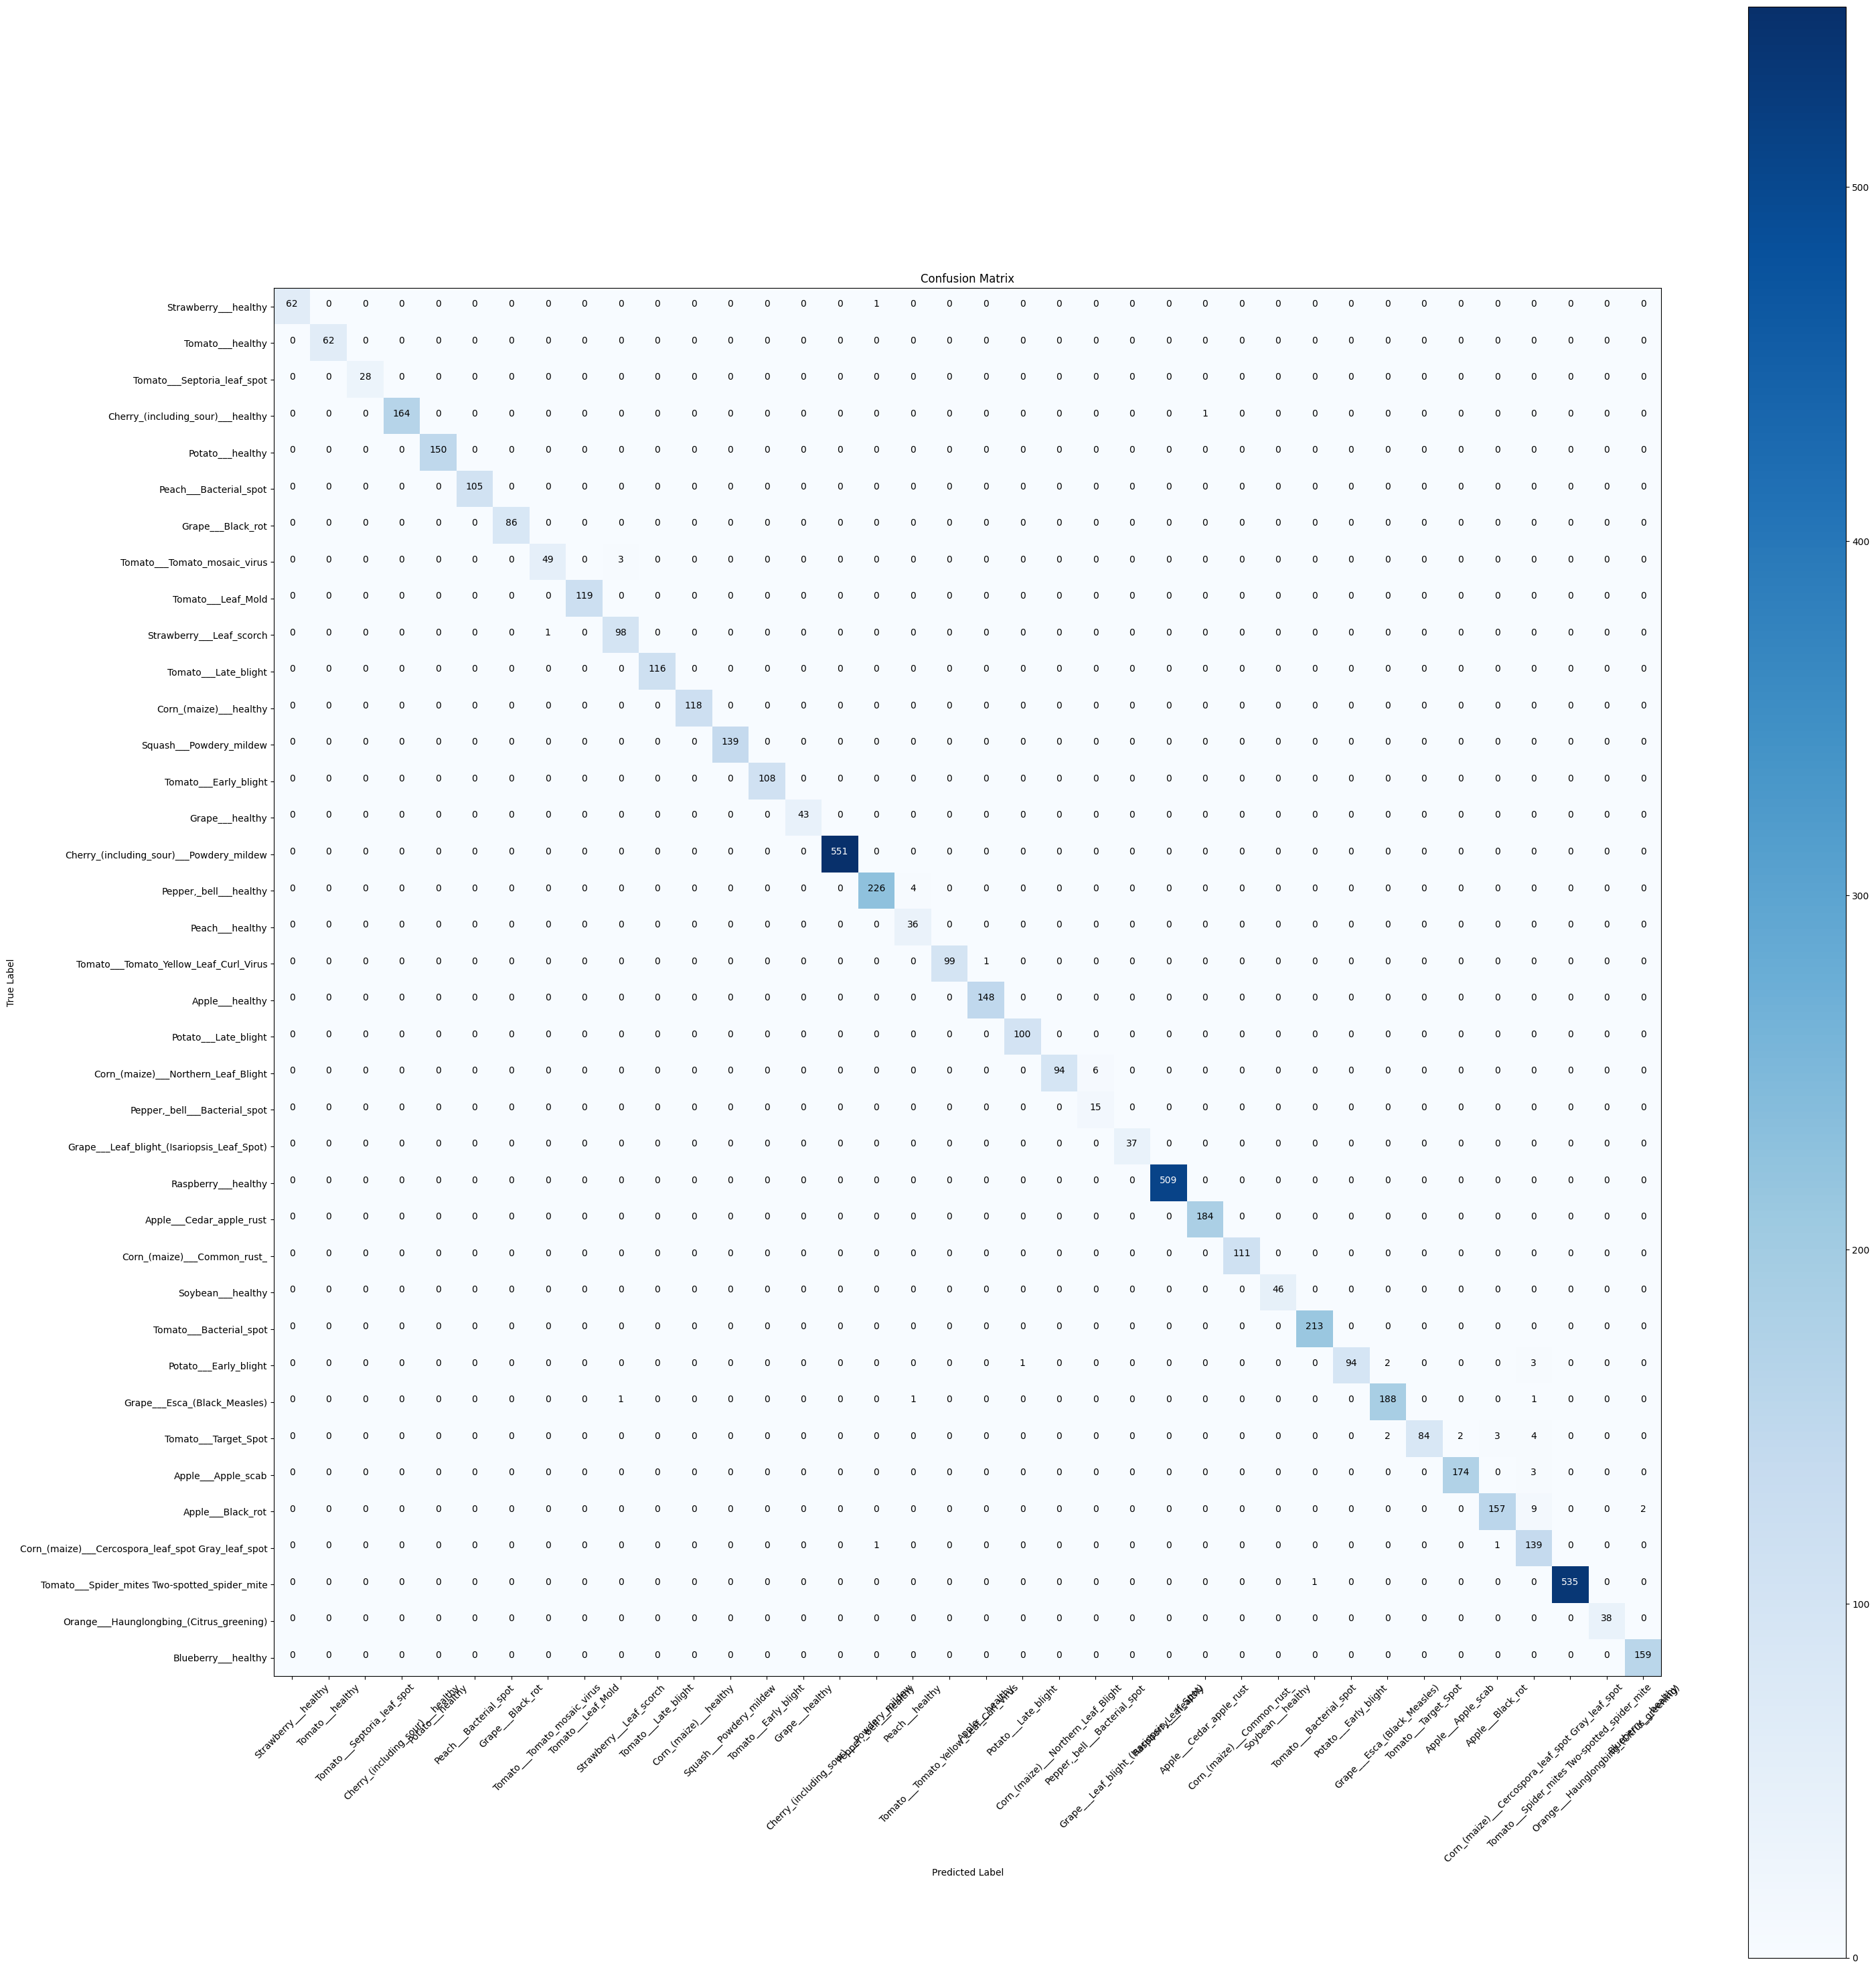
\includegraphics[width= 0.9\textwidth]{assets/FTConfMatrix.png} 
    \caption{Confusion Matrix} 
    \label{fig:immagine}
\end{figure}

Upon examination, it becomes evident that this model has surpassed its predecessor, achieving higher F1-scores and 
accuracy rates for the majority of classes. Impressively, even in the face of limited support for the 
\textit{Pepper\_bell\_Bacterial\_spot} class, the model successfully classifies it with a commendable accuracy score of 83\%.

\section{Conclusion}

In summary, our study highlights the significant advantages of fine-tuning a pre-trained model over building one from 
scratch in the leaf classification task. The fine-tuned model demonstrated exceptional performance, achieving an accuracy
of 99.01\%, which effectively categorizes leaves into multiple classes. While the from-scratch model, while lighter 
in complexity, still achieved a respectable accuracy of 97.59\%, the superior performance of the fine-tuned model 
underscores the value of leveraging pre-trained networks for image classification tasks.

It's crucial to emphasize that the 99.01\% accuracy achieved by the fine-tuned model meets the specific classification 
requirements of our study, ensuring reliable leaf categorization.

Moreover, it's worth noting that both models could have benefited from better support in the test set.

Additionally, we acknowledge that ensemble methods, although not implemented due to resource and time constraints 
in our academic setting, could have potentially further improved our classification results.

In conclusion, our findings underscore the effectiveness of fine-tuning pre-trained models and highlight the practicality 
of achieving impressive accuracy levels in leaf classification

\bibliographystyle{plain}
\bibliography{chapters/Bibliografy.bib}

\end{document}
% --------------------------------------